\documentclass{beamer}\usepackage{graphicx, color}
%% maxwidth is the original width if it is less than linewidth
%% otherwise use linewidth (to make sure the graphics do not exceed the margin)
\makeatletter
\def\maxwidth{ %
  \ifdim\Gin@nat@width>\linewidth
    \linewidth
  \else
    \Gin@nat@width
  \fi
}
\makeatother

\definecolor{fgcolor}{rgb}{0.2, 0.2, 0.2}
\newcommand{\hlnumber}[1]{\textcolor[rgb]{0,0,0}{#1}}%
\newcommand{\hlfunctioncall}[1]{\textcolor[rgb]{0.501960784313725,0,0.329411764705882}{\textbf{#1}}}%
\newcommand{\hlstring}[1]{\textcolor[rgb]{0.6,0.6,1}{#1}}%
\newcommand{\hlkeyword}[1]{\textcolor[rgb]{0,0,0}{\textbf{#1}}}%
\newcommand{\hlargument}[1]{\textcolor[rgb]{0.690196078431373,0.250980392156863,0.0196078431372549}{#1}}%
\newcommand{\hlcomment}[1]{\textcolor[rgb]{0.180392156862745,0.6,0.341176470588235}{#1}}%
\newcommand{\hlroxygencomment}[1]{\textcolor[rgb]{0.43921568627451,0.47843137254902,0.701960784313725}{#1}}%
\newcommand{\hlformalargs}[1]{\textcolor[rgb]{0.690196078431373,0.250980392156863,0.0196078431372549}{#1}}%
\newcommand{\hleqformalargs}[1]{\textcolor[rgb]{0.690196078431373,0.250980392156863,0.0196078431372549}{#1}}%
\newcommand{\hlassignement}[1]{\textcolor[rgb]{0,0,0}{\textbf{#1}}}%
\newcommand{\hlpackage}[1]{\textcolor[rgb]{0.588235294117647,0.709803921568627,0.145098039215686}{#1}}%
\newcommand{\hlslot}[1]{\textit{#1}}%
\newcommand{\hlsymbol}[1]{\textcolor[rgb]{0,0,0}{#1}}%
\newcommand{\hlprompt}[1]{\textcolor[rgb]{0.2,0.2,0.2}{#1}}%

\usepackage{framed}
\makeatletter
\newenvironment{kframe}{%
 \def\at@end@of@kframe{}%
 \ifinner\ifhmode%
  \def\at@end@of@kframe{\end{minipage}}%
  \begin{minipage}{\columnwidth}%
 \fi\fi%
 \def\FrameCommand##1{\hskip\@totalleftmargin \hskip-\fboxsep
 \colorbox{shadecolor}{##1}\hskip-\fboxsep
     % There is no \\@totalrightmargin, so:
     \hskip-\linewidth \hskip-\@totalleftmargin \hskip\columnwidth}%
 \MakeFramed {\advance\hsize-\width
   \@totalleftmargin\z@ \linewidth\hsize
   \@setminipage}}%
 {\par\unskip\endMakeFramed%
 \at@end@of@kframe}
\makeatother

\definecolor{shadecolor}{rgb}{.97, .97, .97}
\definecolor{messagecolor}{rgb}{0, 0, 0}
\definecolor{warningcolor}{rgb}{1, 0, 1}
\definecolor{errorcolor}{rgb}{1, 0, 0}
\newenvironment{knitrout}{}{} % an empty environment to be redefined in TeX

\usepackage{alltt}
\usepackage{amsmath, amsthm}
\usepackage{parskip, microtype, graphicx, caption, multirow}

\frenchspacing  % i likes it







\title{How cryptic is cryptic diversity? \newline Machine learning approaches to fine scale variation in the morphology of \textit{Emys marmorata}.}
\author[shortname]{Peter D Smits\inst{1}, 
                   Kenneth D Angielczyk\inst{2}, 
                   James F Parham\inst{3}}
\institute[shortinst]{\inst{1} Committee on Evolution Biology, University of Chicago,
                      \inst{2} Department of Geology, Field Museum of Natural History,
                      \inst{3} Department of Geological Sciences, California State University -- Fullerton}
\IfFileExists{upquote.sty}{\usepackage{upquote}}{}

\begin{document}

\begin{frame}
  \maketitle
\end{frame}


\section{Introduction}
\begin{frame}
  \frametitle{Cryptic diversity}
  % image of example taxa that are morphologically identical and are only differentiated via genetic means
  %
  Crytic species are species delimitated via molecular means which were not/cannot be identified via morphology.

  How much of cryptic diversity is just a function of sample size and/or method?

\end{frame}

\begin{frame}
  \frametitle{\textit{Emys marmorata}}
  % picture of a turtle
  % this is the study system
  % a little natural history
  % a little biogeography
  \begin{figure}[h]
    \centering
    \captionsetup{justification = raggedleft, slc = off}
    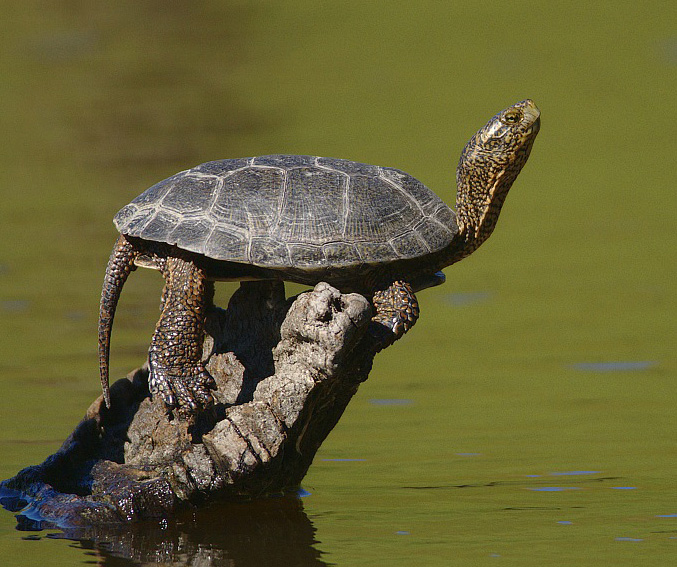
\includegraphics[width = 0.8\textwidth, keepaspectratio = true]{figure/turtle}
    \caption*{wikimedia}
    \label{fig:turtle}
  \end{figure}
\end{frame}

\begin{frame}
  \frametitle{Morphological hypotheses}
\end{frame}

\begin{frame}
  \frametitle{Phylogenetic hypotheses}

  % Number of subspecies and where they occur.
  % images of the different phylobiogeographic hypotheses from the different spinks papers
 
\end{frame}


\section{Methods}
\begin{frame}
  \frametitle{Methods: morphometrics}
  \begin{columns}
    \begin{column}{0.5\textwidth}
      \begin{itemize}
        %\item nrow(turtle.adult) adult individuals
        \item plastral (``belly'') shape
        \item landmarks averaged across bilat axis
        \item total 13 landmarks, 7 on bilat axis, 6 off
        \item geographic information known/inferred
      \end{itemize}
    \end{column}
    \begin{column}{0.5\textwidth}
      \begin{figure}[h]
        \centering
        \captionsetup{justification = raggedleft, slc = off}
        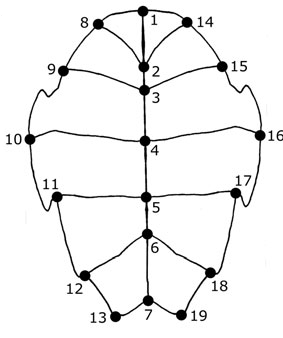
\includegraphics[width = \textwidth, keepaspectratio = true]{figure/plastra}
        \caption*{\scriptsize{Angielczyk \textit{et al.} 2011 \textit{Evolution}}}
        \label{fig:plast}
      \end{figure}
    \end{column}
  \end{columns}
\end{frame}

\begin{frame}
  \frametitle{Unsupervised learning}

  Fancy way of saying clustering or density estimation.

  Partitioning around mediods (PAM) compared with ``gap'' statistic.

  (dissimilarity based) Evidence accumulation clustering
\end{frame}

\begin{frame}
  \frametitle{Supervised learning}

  Fancy way of saying classification and regression.

  Here, features (principal components) predict class (subspecific assignment).

  Multinomial logistic regression

  Random forests
\end{frame}

\begin{frame}
  \frametitle{Model training and selection}
  Unknown appropriate number of features to ``best'' predict class. Want to minimize false positive, while maximizing true positive.

  Split data set, 75-25, training and testing.

  Tuning parameters via grid-search. Uncertainty via 10-fold cross-validation. Selection viamax AUC ROC.

  Best multinomial logistic model selected via min AICc. Best random forest model via max AUC ROC.

\end{frame}

\begin{frame}
  \frametitle{ROC and confusion matrices}

  \begin{center}
    \begin{tabular}[c]{ p{2cm} c | p{2cm} | p{2cm} |}
      \cline{3-4} 
      & & \multicolumn{2}{ c |}{Predicted class} \\ \cline{3-4}
      & & 1 & 0 \\ \hline
      \multicolumn{1}{| c |}{\multirow{2}{*}{Actual class}}
      & 1 & TRUE \newline POSITIVE & FALSE \newline NEGATIVE \\ \cline{2-4}
      \multicolumn{1}{| c |}{} & 0 & FALSE \newline POSITIVE & TRUE \newline NEGATIVE \\
      \hline
    \end{tabular}
  \end{center}

\end{frame}

\begin{frame}
  \frametitle{ROC}
  \begin{columns}
    \begin{column}{0.4\textwidth}
      \begin{itemize}
        \item receiver operating characteristic
        \item true positive rate or sensitivity: \(\frac{TP}{TP + FN}\)
        \item false positive rate or \newline 1 - specificity: \(\frac{FP}{FP + TN}\)
        \item multiclass, all-against one (Hand and Till 2001 \textit{Machine Learning})
        \item area under curve model summary statistic (min 0.5)
      \end{itemize}
    \end{column}
    \begin{column}{0.6\textwidth}
      \begin{figure}[h]
        \centering
        \captionsetup{justification = raggedleft, slc = off}
        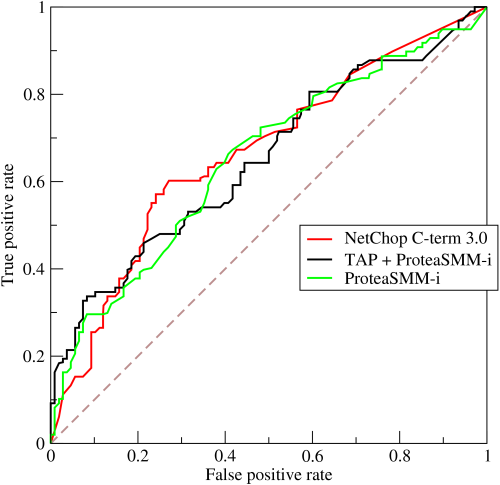
\includegraphics[width = \textwidth, keepaspectratio = true]{figure/wiki_roc}
        \caption*{\scriptsize{wikimedia}}
        \label{fig:roc}
      \end{figure}
    \end{column}
  \end{columns}

\end{frame}


\section{Results}
\begin{frame}[fragile]
  \frametitle{Results: mophometrics}
\begin{knitrout}
\definecolor{shadecolor}{rgb}{1, 1, 1}\color{fgcolor}
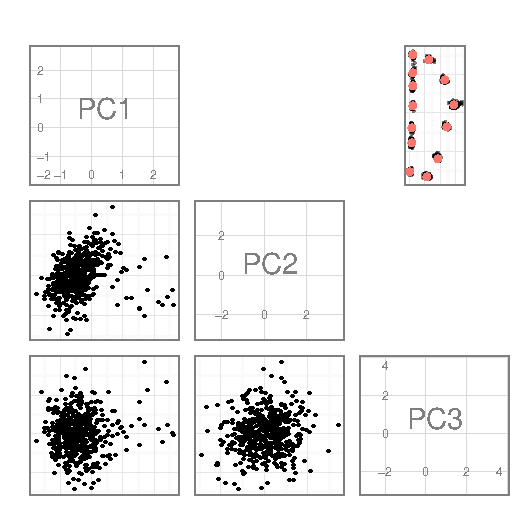
\includegraphics[width=\maxwidth]{figure/gm} 

\end{knitrout}


\end{frame}

\begin{frame}[fragile]
  \frametitle{Results: gap clustering}
\begin{knitrout}
\definecolor{shadecolor}{rgb}{1, 1, 1}\color{fgcolor}
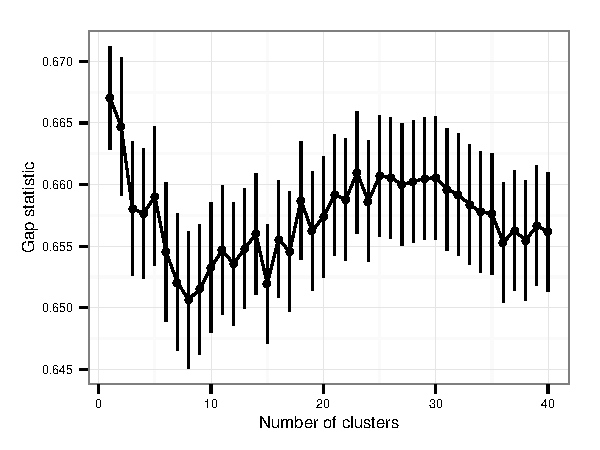
\includegraphics[width=\maxwidth]{figure/gap} 

\end{knitrout}

\end{frame}

\begin{frame}
  \frametitle{Results: d-EAC}

\end{frame}

% model selection is unnecessary because of time constraints
\begin{frame}[fragile]
  \frametitle{ROC}
\begin{knitrout}
\definecolor{shadecolor}{rgb}{1, 1, 1}\color{fgcolor}
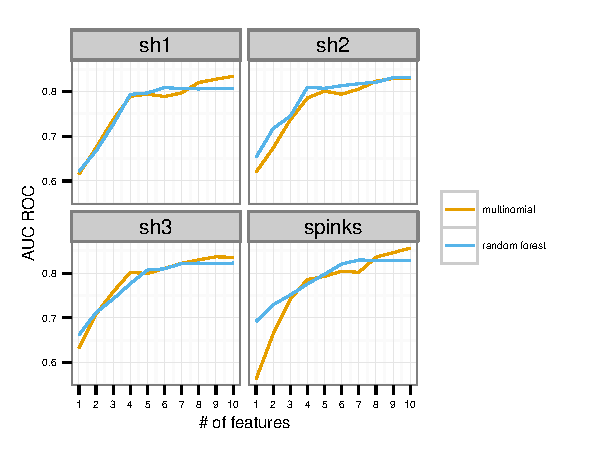
\includegraphics[width=\maxwidth]{figure/roc} 

\end{knitrout}


\end{frame}

\begin{frame}
  \frametitle{Are the AUC ROC values meaningful?}
\end{frame}


\begin{frame}
  \frametitle{Best classification scheme?}
\end{frame}

\begin{frame}[fragile]
  \frametitle{Variable importance}
  % ggpairs from the best random forest model
\begin{knitrout}
\definecolor{shadecolor}{rgb}{1, 1, 1}\color{fgcolor}
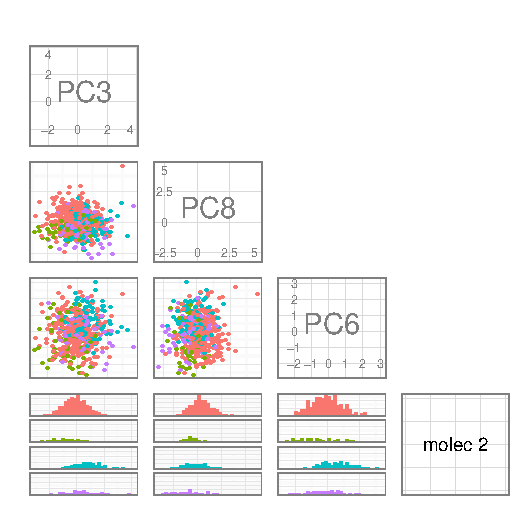
\includegraphics[width=\maxwidth]{figure/imp} 

\end{knitrout}

\end{frame}

\section{Discussion}
\begin{frame}
  \frametitle{Future}
\end{frame}

\begin{frame}
  \frametitle{Acknowledgements}
  \begin{columns}
    \begin{column}{0.5\textwidth}
      \begin{itemize}
        \item Ben Frable, Dallas Krentzel, Michael Foote
        \item COLLECTIONS
        \item FUNDING AGENCIES
      \end{itemize}
    \end{column}
    \begin{column}{0.5\textwidth}
      
\includegraphics[height = 0.25\textheight, keepaspectratio = true]{figure/chicago} \\
      
\includegraphics[height = 0.25\textheight, width = \textwidth, keepaspectratio = true]{figure/field} \\
      
\includegraphics[height = 0.25\textheight, keepaspectratio = true]{figure/csu}
    \end{column}
  \end{columns}
\end{frame}
\end{document}
